
\begin{appendix}

\chapter{Meetings}\label{ch:Meetings}
The following tables are showing the protocolls of the held team meetings.

\begin{figure}
  \centering
    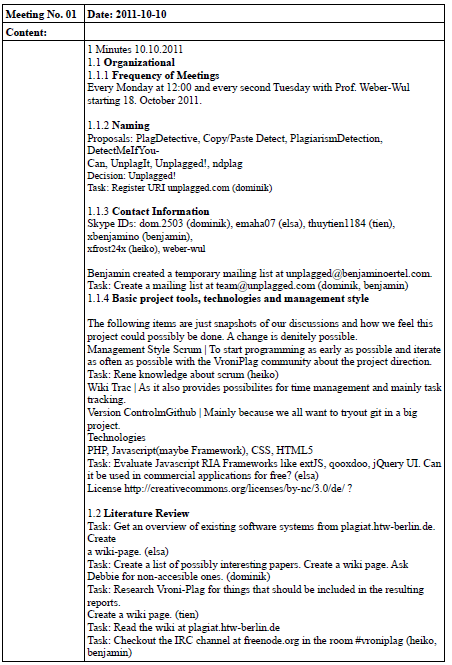
\includegraphics[width=\textwidth]{images/a_meetings/meeting_01a.png}
  \caption{Meeting protocol no. 1 part 1}
  \label{fig:meeting protocol no. 1 part 1}
\end{figure}

\begin{figure}
  \centering
    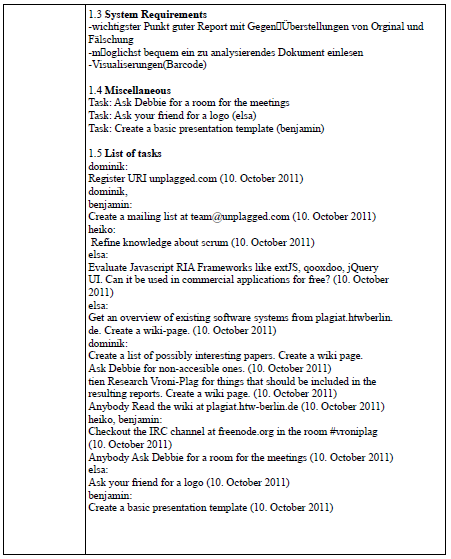
\includegraphics[width=\textwidth]{images/a_meetings/meeting_01b.png}
  \caption{Meeting protocol no. 1 part 2}
  \label{fig:meeting protocol no. 1 part 2}
\end{figure}

\begin{figure}
  \centering
    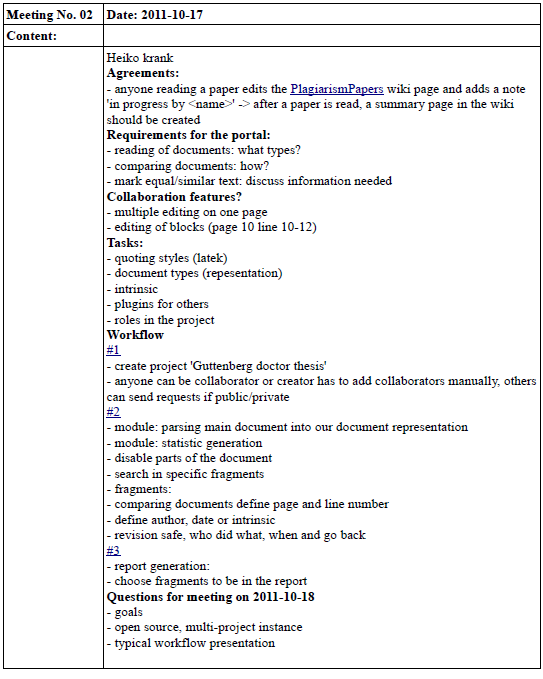
\includegraphics[width=\textwidth]{images/a_meetings/meeting_02.png}
  \caption{Meeting protocol no. 2}
  \label{fig:meeting protocol no. 2}
\end{figure}

\begin{figure}
  \centering
    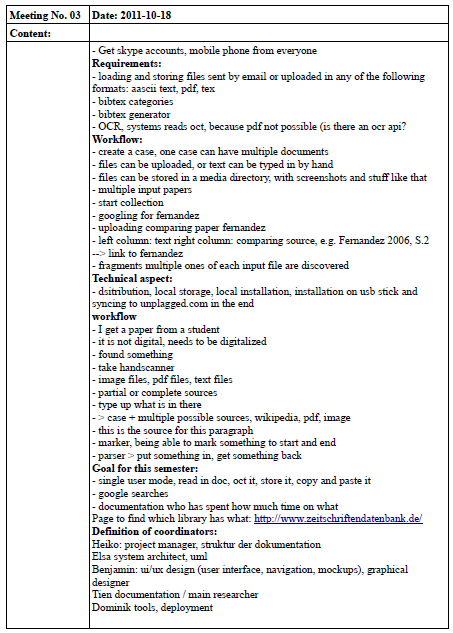
\includegraphics[width=\textwidth]{images/a_meetings/meeting_03.png}
  \caption{Meeting protocol no. 3}
  \label{fig:meeting protocol no. 3}
\end{figure}

\begin{figure}
  \centering
    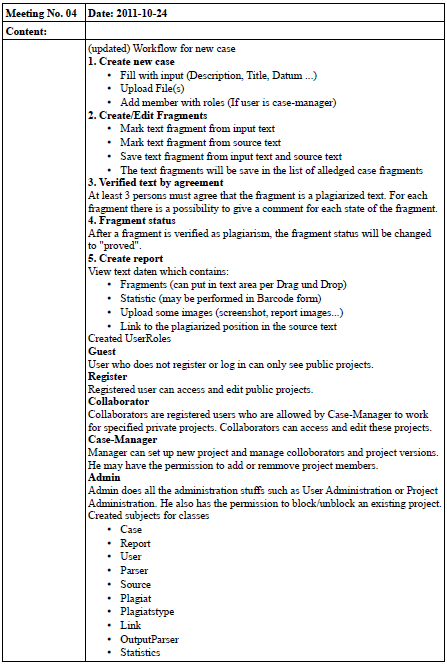
\includegraphics[width=\textwidth]{images/a_meetings/meeting_04a.png}
  \caption{Meeting protocol no. 4 part 1}
  \label{fig:meeting protocol no. 4 part 1}
\end{figure}

\begin{figure}
  \centering
    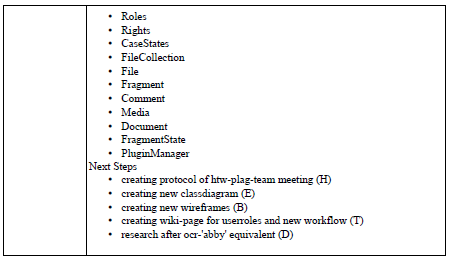
\includegraphics[width=\textwidth]{images/a_meetings/meeting_04b.png}
  \caption{Meeting protocol no. 4 part 2}
  \label{fig:meeting protocol no. 4 part 2}
\end{figure}

\begin{figure}
  \centering
    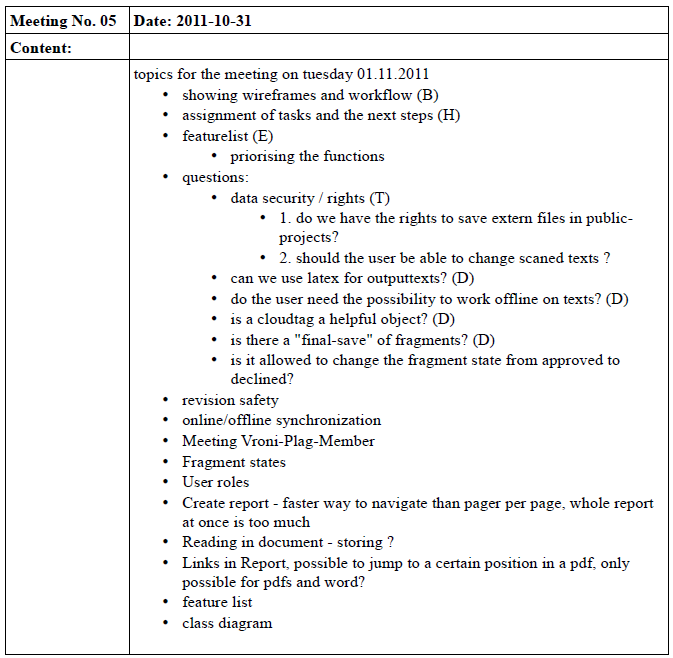
\includegraphics[width=\textwidth]{images/a_meetings/meeting_05.png}
  \caption{Meeting protocol no 5}
  \label{fig:meeting protocol no. 5}
\end{figure}

\begin{figure}
  \centering
    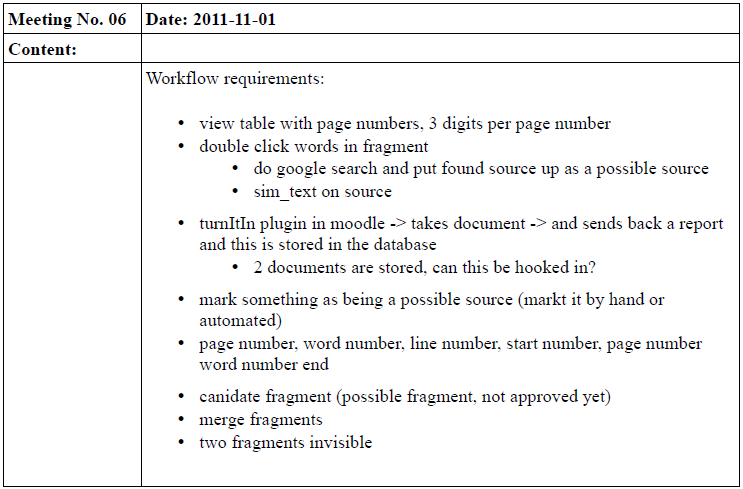
\includegraphics[width=\textwidth]{images/a_meetings/meeting_06.png}
  \caption{Meeting protocol no 6}
  \label{fig:meeting protocol no. 6}
\end{figure}

\begin{figure}
  \centering
    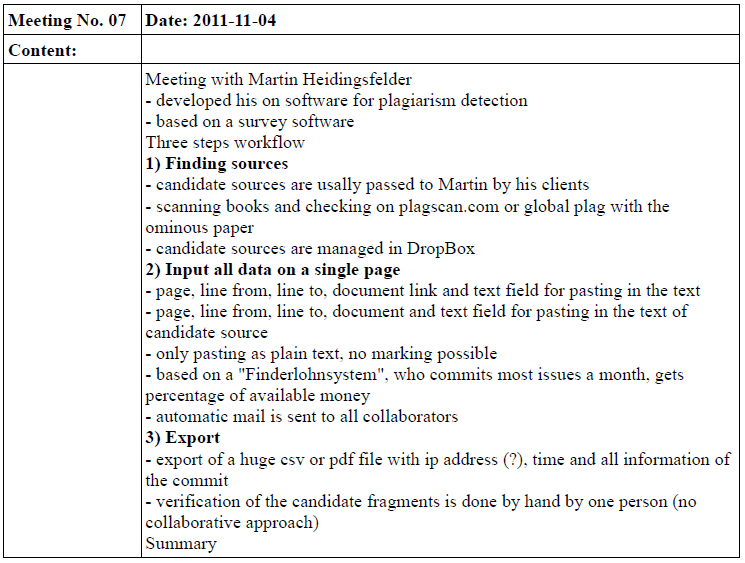
\includegraphics[width=\textwidth]{images/a_meetings/meeting_07.png}
  \caption{Meeting protocol no. 7}
  \label{fig:meeting protocol no. 7}
\end{figure}

\begin{figure}
  \centering
    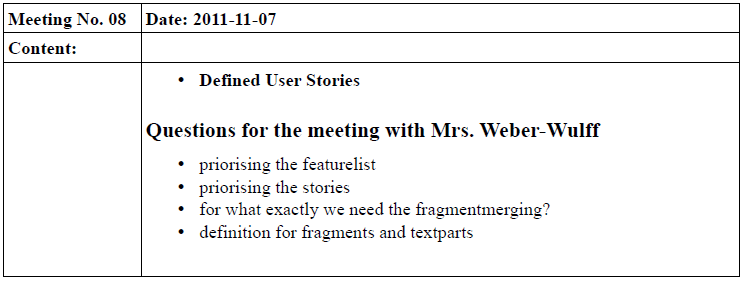
\includegraphics[width=\textwidth]{images/a_meetings/meeting_08.png}
  \caption{Meeting protocol no. 8}
  \label{fig:meeting protocol no. 8}
\end{figure}

\begin{figure}
  \centering
    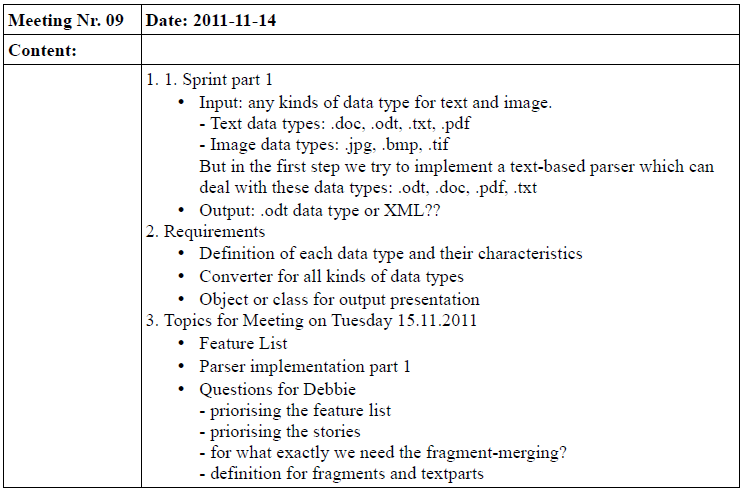
\includegraphics[width=\textwidth]{images/a_meetings/meeting_09.png}
  \caption{Meeting protocol no. 9}
  \label{fig:meeting protocol no. 9}
\end{figure}

\begin{figure}
  \centering
    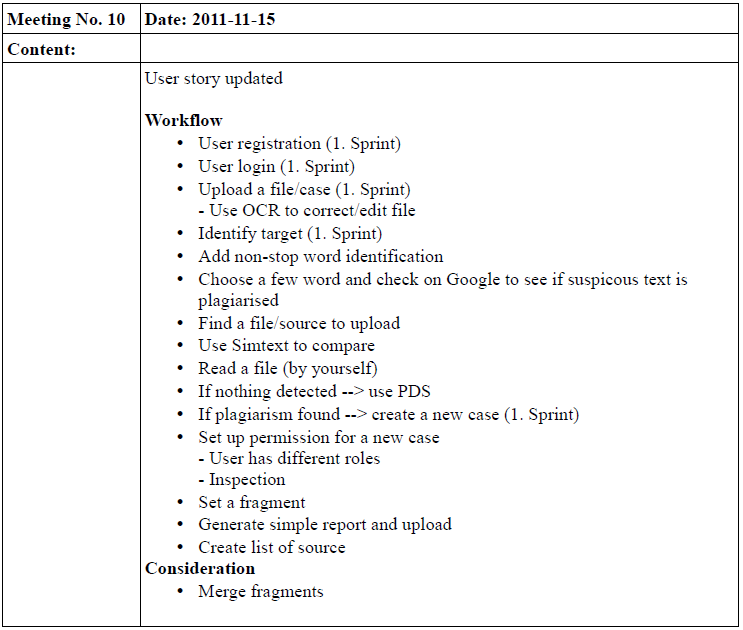
\includegraphics[width=\textwidth]{images/a_meetings/meeting_10.png}
  \caption{Meeting protocol no. 10}
  \label{fig:meeting protocol no. 10}
\end{figure}

\begin{figure}
  \centering
    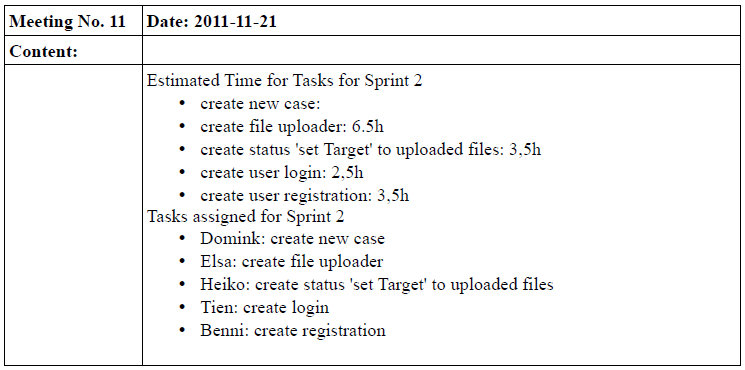
\includegraphics[width=\textwidth]{images/a_meetings/meeting_11.png}
  \caption{Meeting protocol no. 11}
  \label{fig:meeting protocol no. 11}
\end{figure}

\begin{figure}
  \centering
    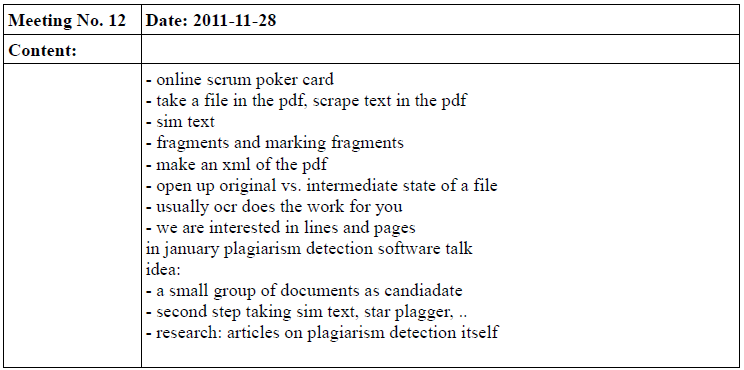
\includegraphics[width=\textwidth]{images/a_meetings/meeting_12.png}
  \caption{Meeting protocol no. 12}
  \label{fig:meeting protocol no. 12}
\end{figure}

\begin{figure}
  \centering
    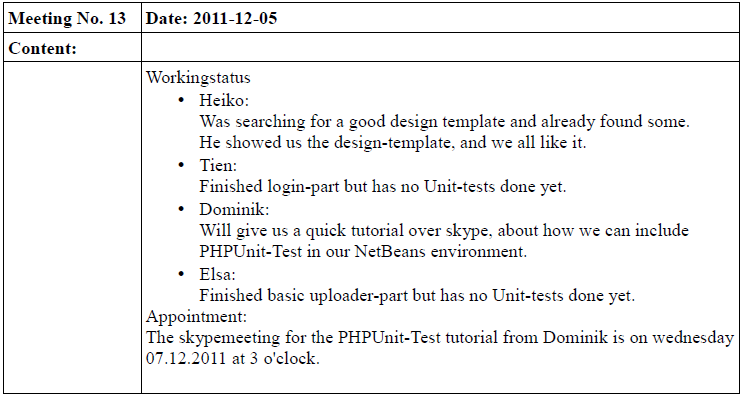
\includegraphics[width=\textwidth]{images/a_meetings/meeting_13.png}
  \caption{Meeting protocol no. 13}
  \label{fig:meeting protocol no. 13}
\end{figure}
\clearpage
\begin{figure}
  \centering
    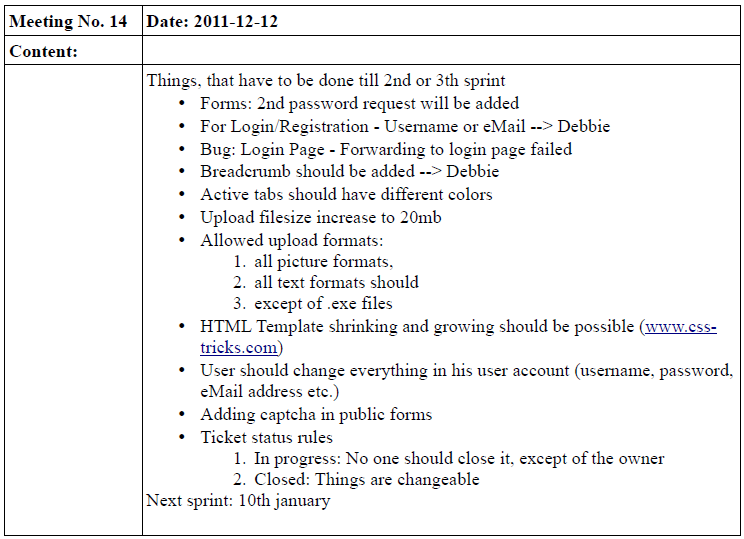
\includegraphics[width=\textwidth]{images/a_meetings/meeting_14.png}
  \caption{Meeting protocol no. 14}
  \label{fig:meeting protocol no. 14}
\end{figure}

\begin{figure}
  \centering
    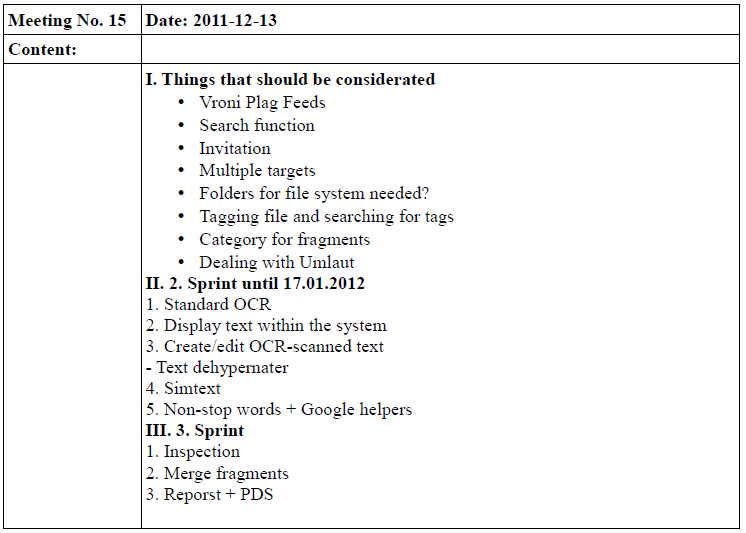
\includegraphics[width=\textwidth]{images/a_meetings/meeting_15.png}
  \caption{Meeting protocol no. 15}
  \label{fig:meeting protocol no. 15}
\end{figure}

\begin{figure}
  \centering
    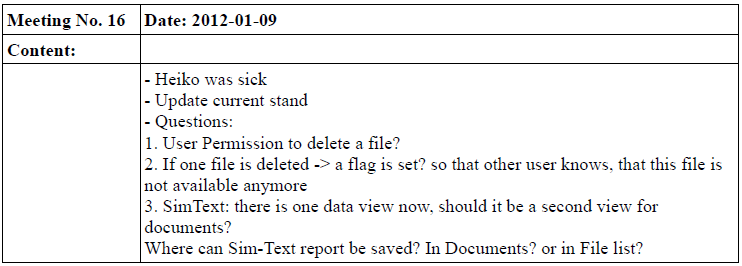
\includegraphics[width=\textwidth]{images/a_meetings/meeting_16.png}
  \caption{Meeting protocol no. 16}
  \label{fig:meeting protocol no. 16}
\end{figure}

\begin{figure}
  \centering
    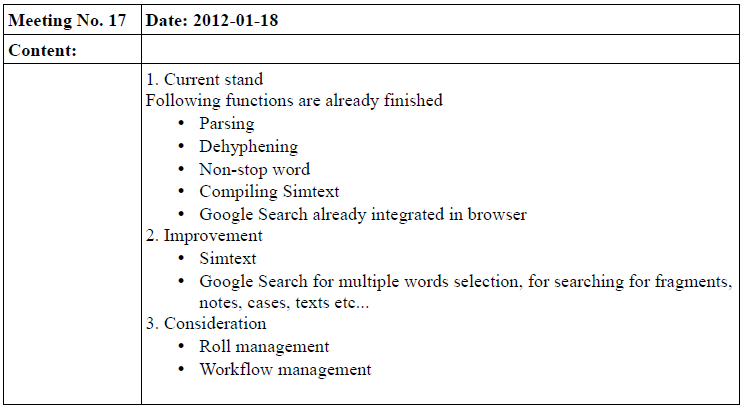
\includegraphics[width=\textwidth]{images/a_meetings/meeting_17.png}
  \caption{Meeting protocol no. 17}
  \label{fig:meeting protocol no. 17}
\end{figure}

\begin{figure}
  \centering
    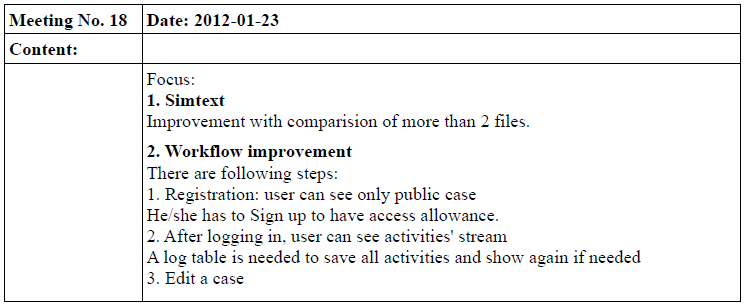
\includegraphics[width=\textwidth]{images/a_meetings/meeting_18.png}
  \caption{Meeting protocol no. 18}
  \label{fig:meeting protocol no. 18}
\end{figure}

\begin{figure}
  \centering
    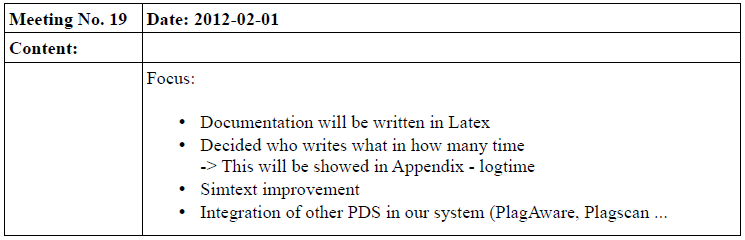
\includegraphics[width=\textwidth]{images/a_meetings/meeting_19.png}
  \caption{Meeting protocol no. 19}
  \label{fig:meeting protocol no. 19}
\end{figure}



\chapter{Logged Time As Of March 11, 2012}

The following tables are some example reports generated from the logged time in Redmine. To find the most recent version
of these reports or to generate custom data analysis you can use the \enquote{Report} tool found in Redmine on the \enquote{Overview}
page.

% should be updated later on, now simply to make sure it works
% generate various reports in redmine and export as csv
% don't forget to escape special characters like _ or # in the input .csv, e. g. \_ or \#

\DTLloaddb{overview}{data/timelog-overview.csv}
\begin{table}[!h]
  \caption{Overview By Member and Month}
  \centering
  \DTLdisplaydb{overview}
\end{table}

\begin{landscape}

\DTLsetseparator{,}

\DTLloaddb{issueMember}{data/timelog-issue-member.csv}
  \centering
 \DTLdisplaylongdb[caption=Overview By Member and Issue]{issueMember}

\DTLloaddb{sprints}{data/timelog-sprints.csv}
\begin{table}[tbp]
  \caption{Overview By Sprints}
  \centering
  \DTLdisplaydb{sprints}
\end{table}

\end{landscape}

\chapter{Mockups}\label{appendix:mockups}

\section{Hand-Drawn}

\begin{figure}[tbp]
  \centering
    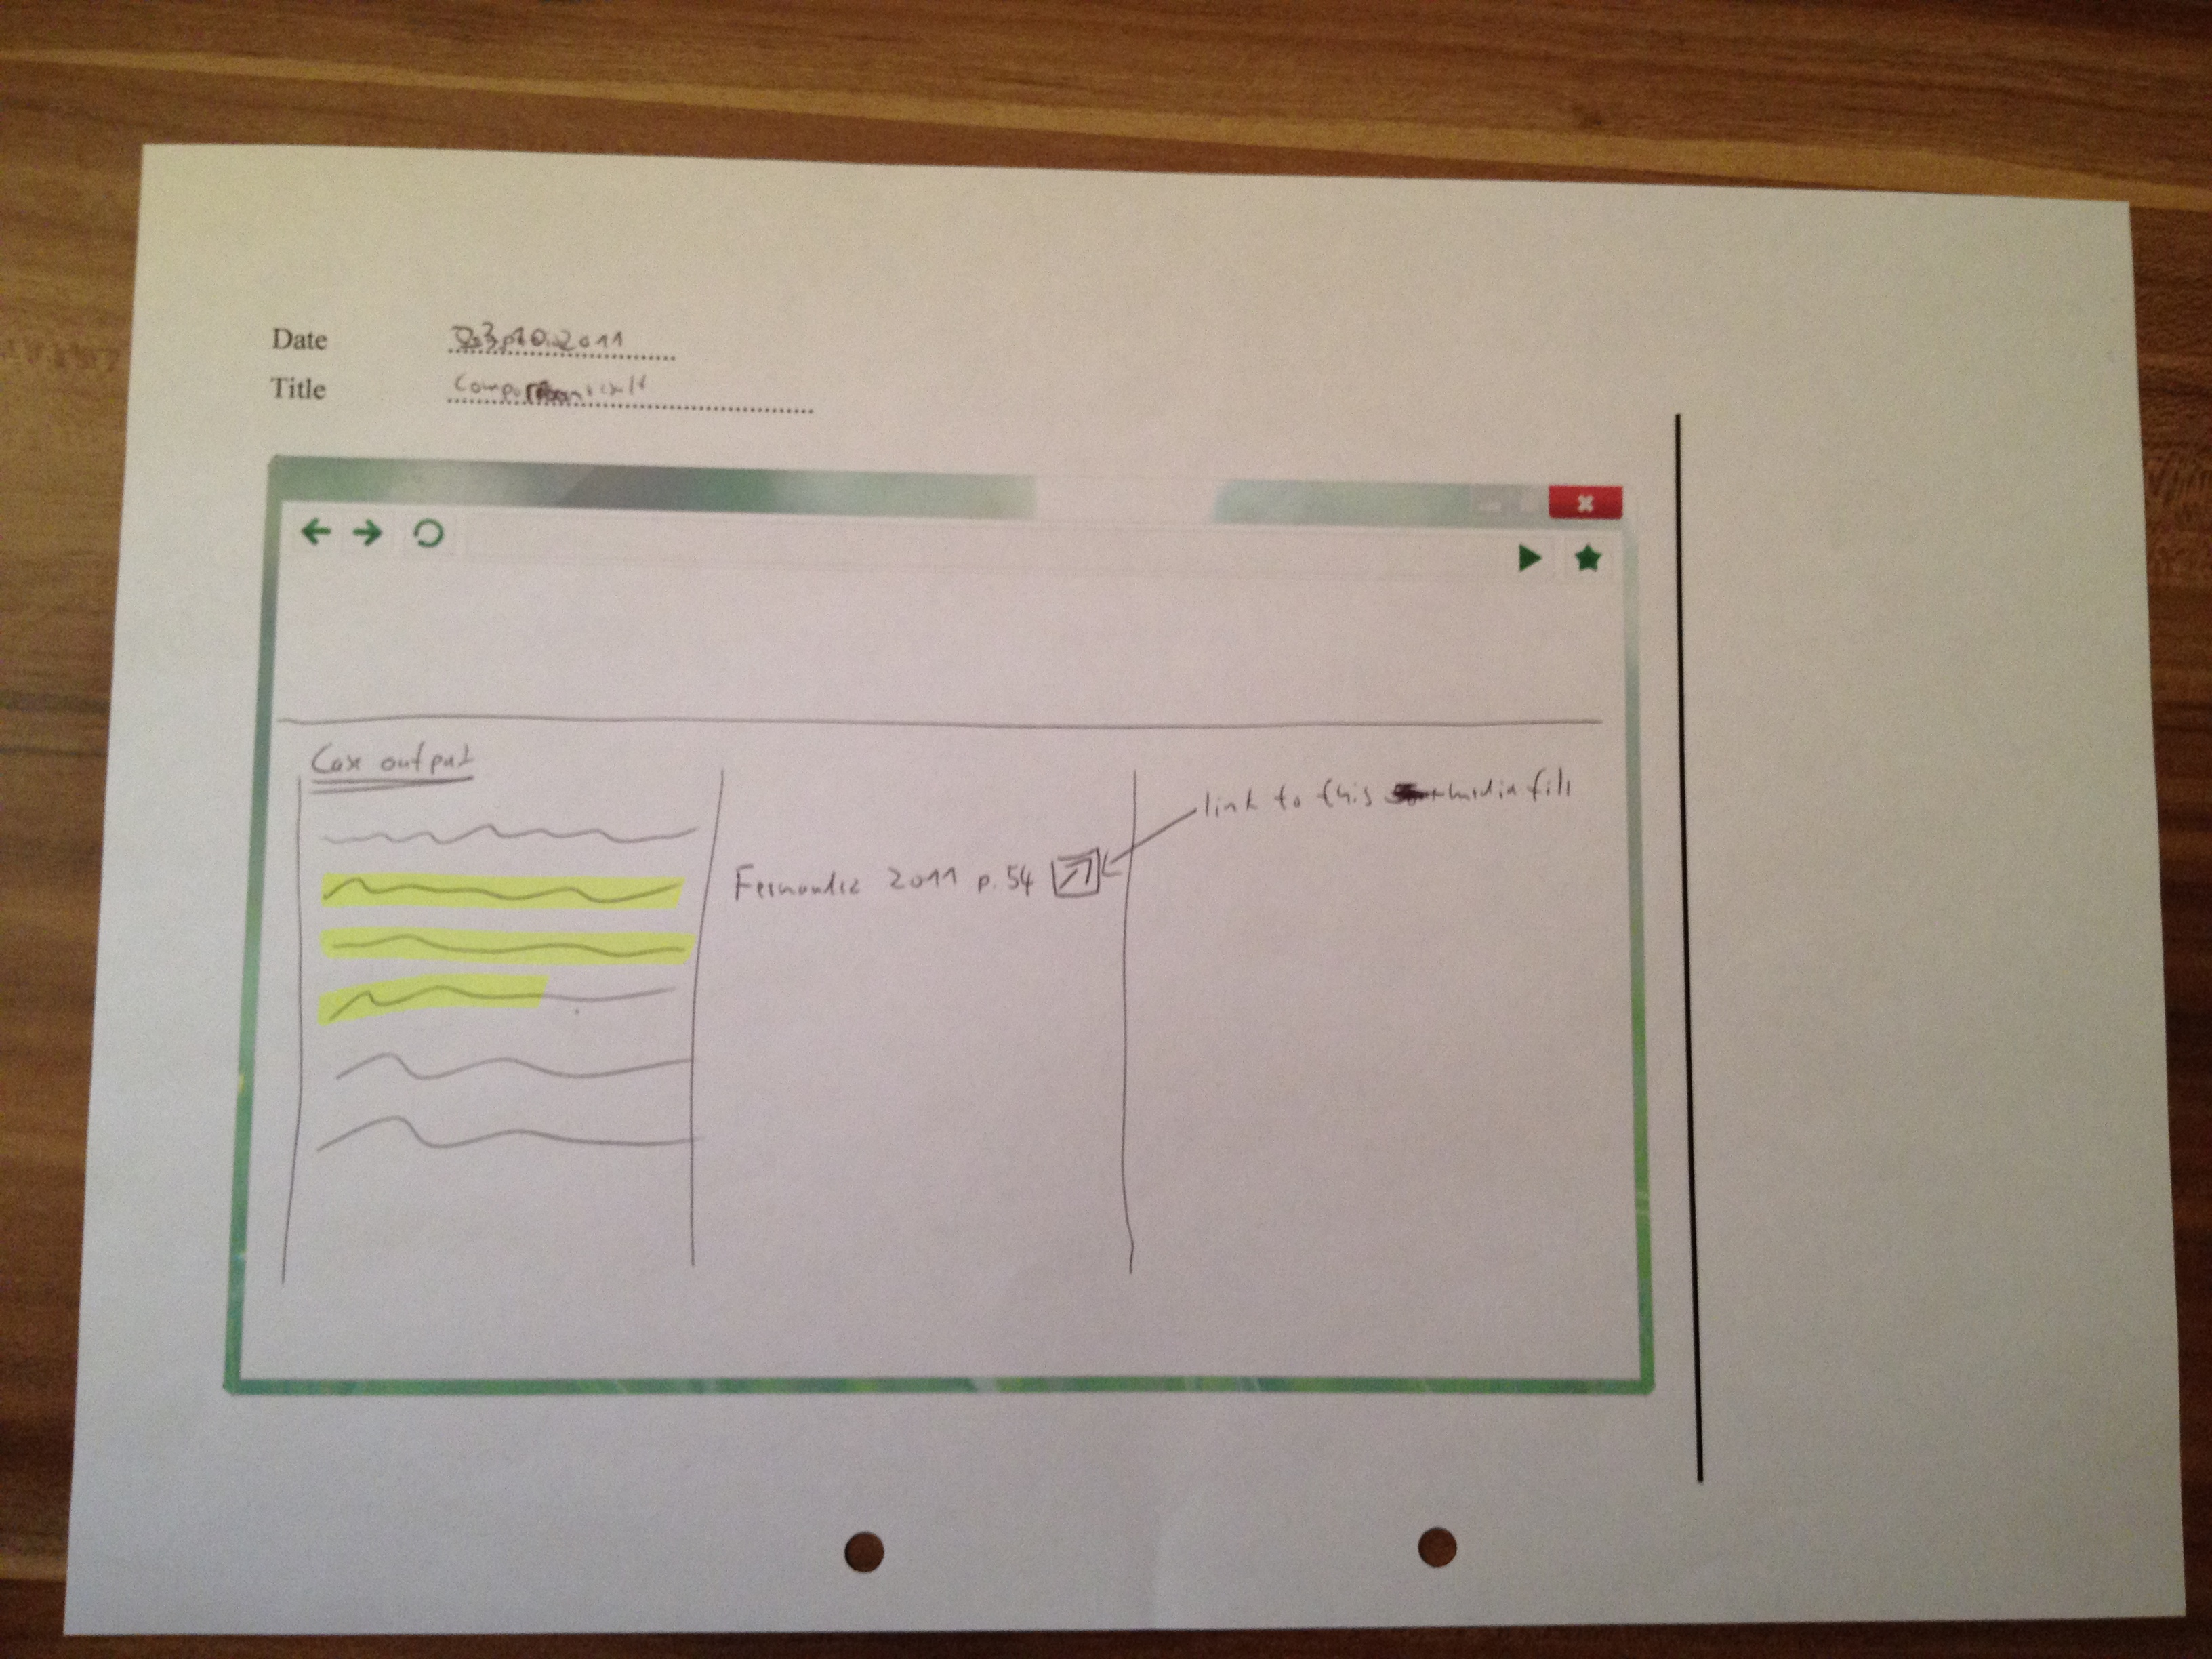
\includegraphics[width=\textwidth]{mockups/m_compare_result.jpg}
  \caption{Mockup – Compare results – digitalized }
  \label{fig:mCompareResultsMockup}
\end{figure}

\begin{figure}[tbp]
  \centering
    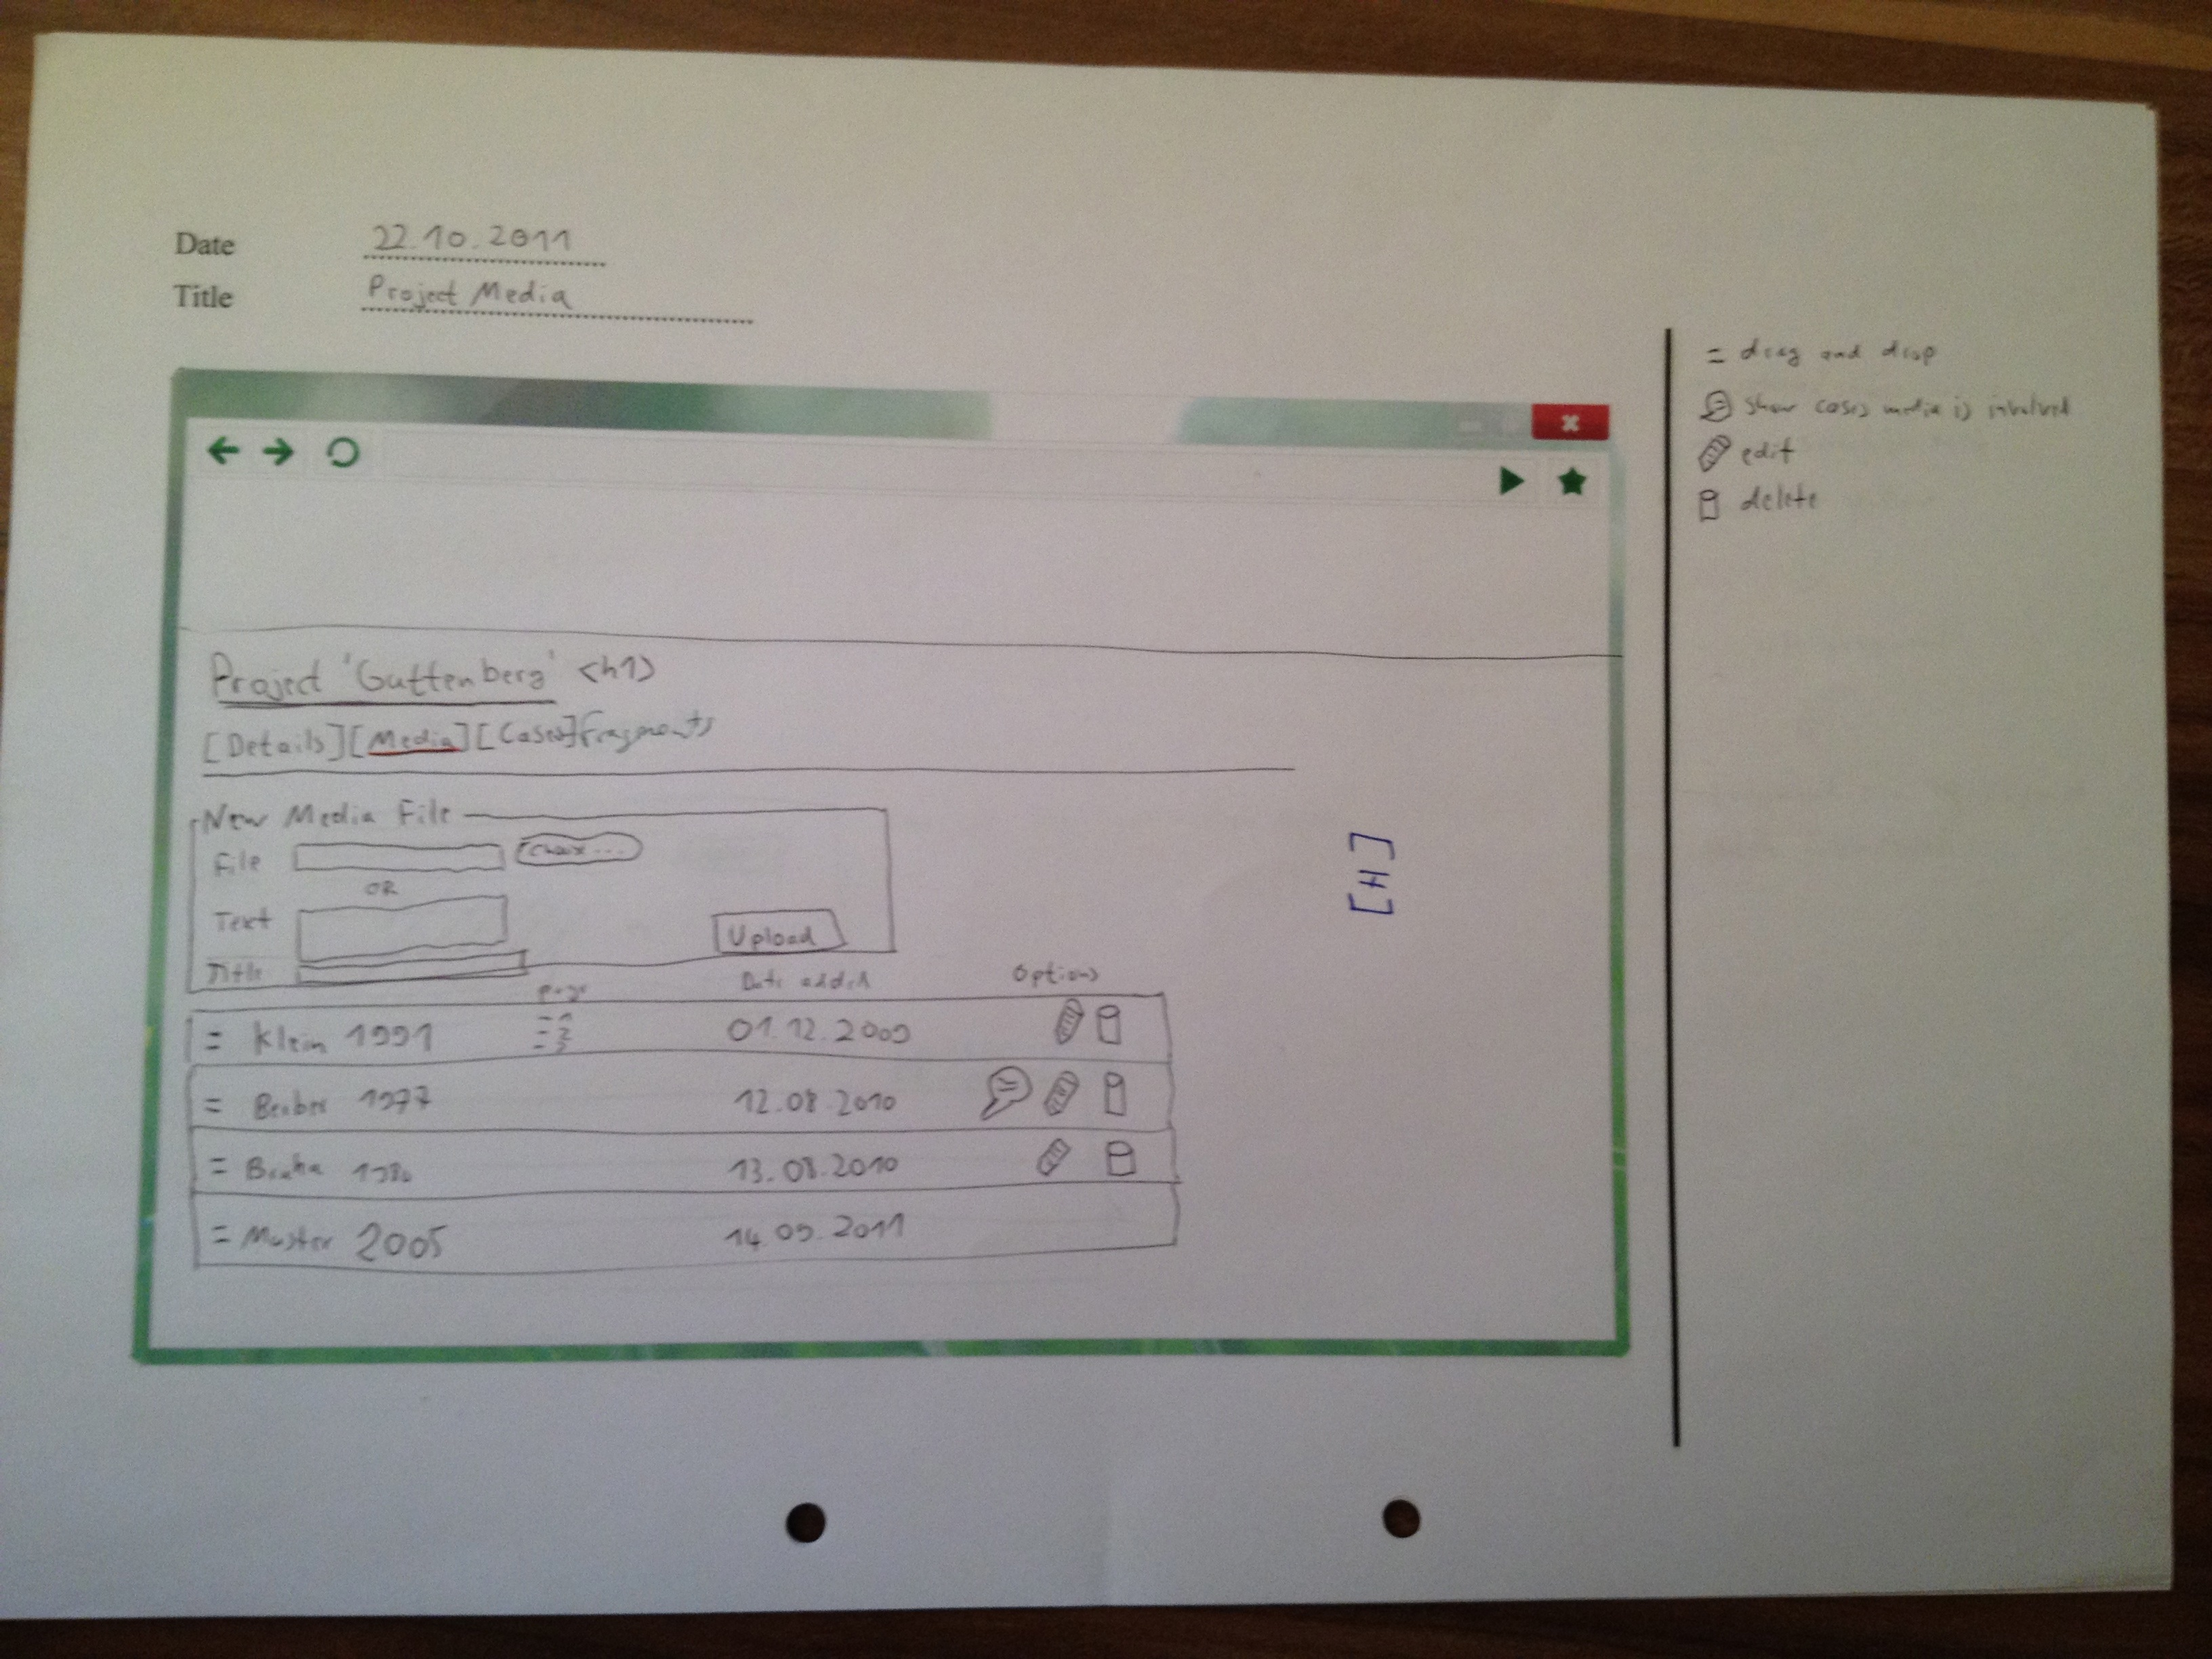
\includegraphics[width=\textwidth]{mockups/m_media_list.jpg}
  \caption{Mockup – Media list – digitalized }
  \label{fig:mMediaListMockup}
\end{figure}

\begin{figure}[tbp]
  \centering
    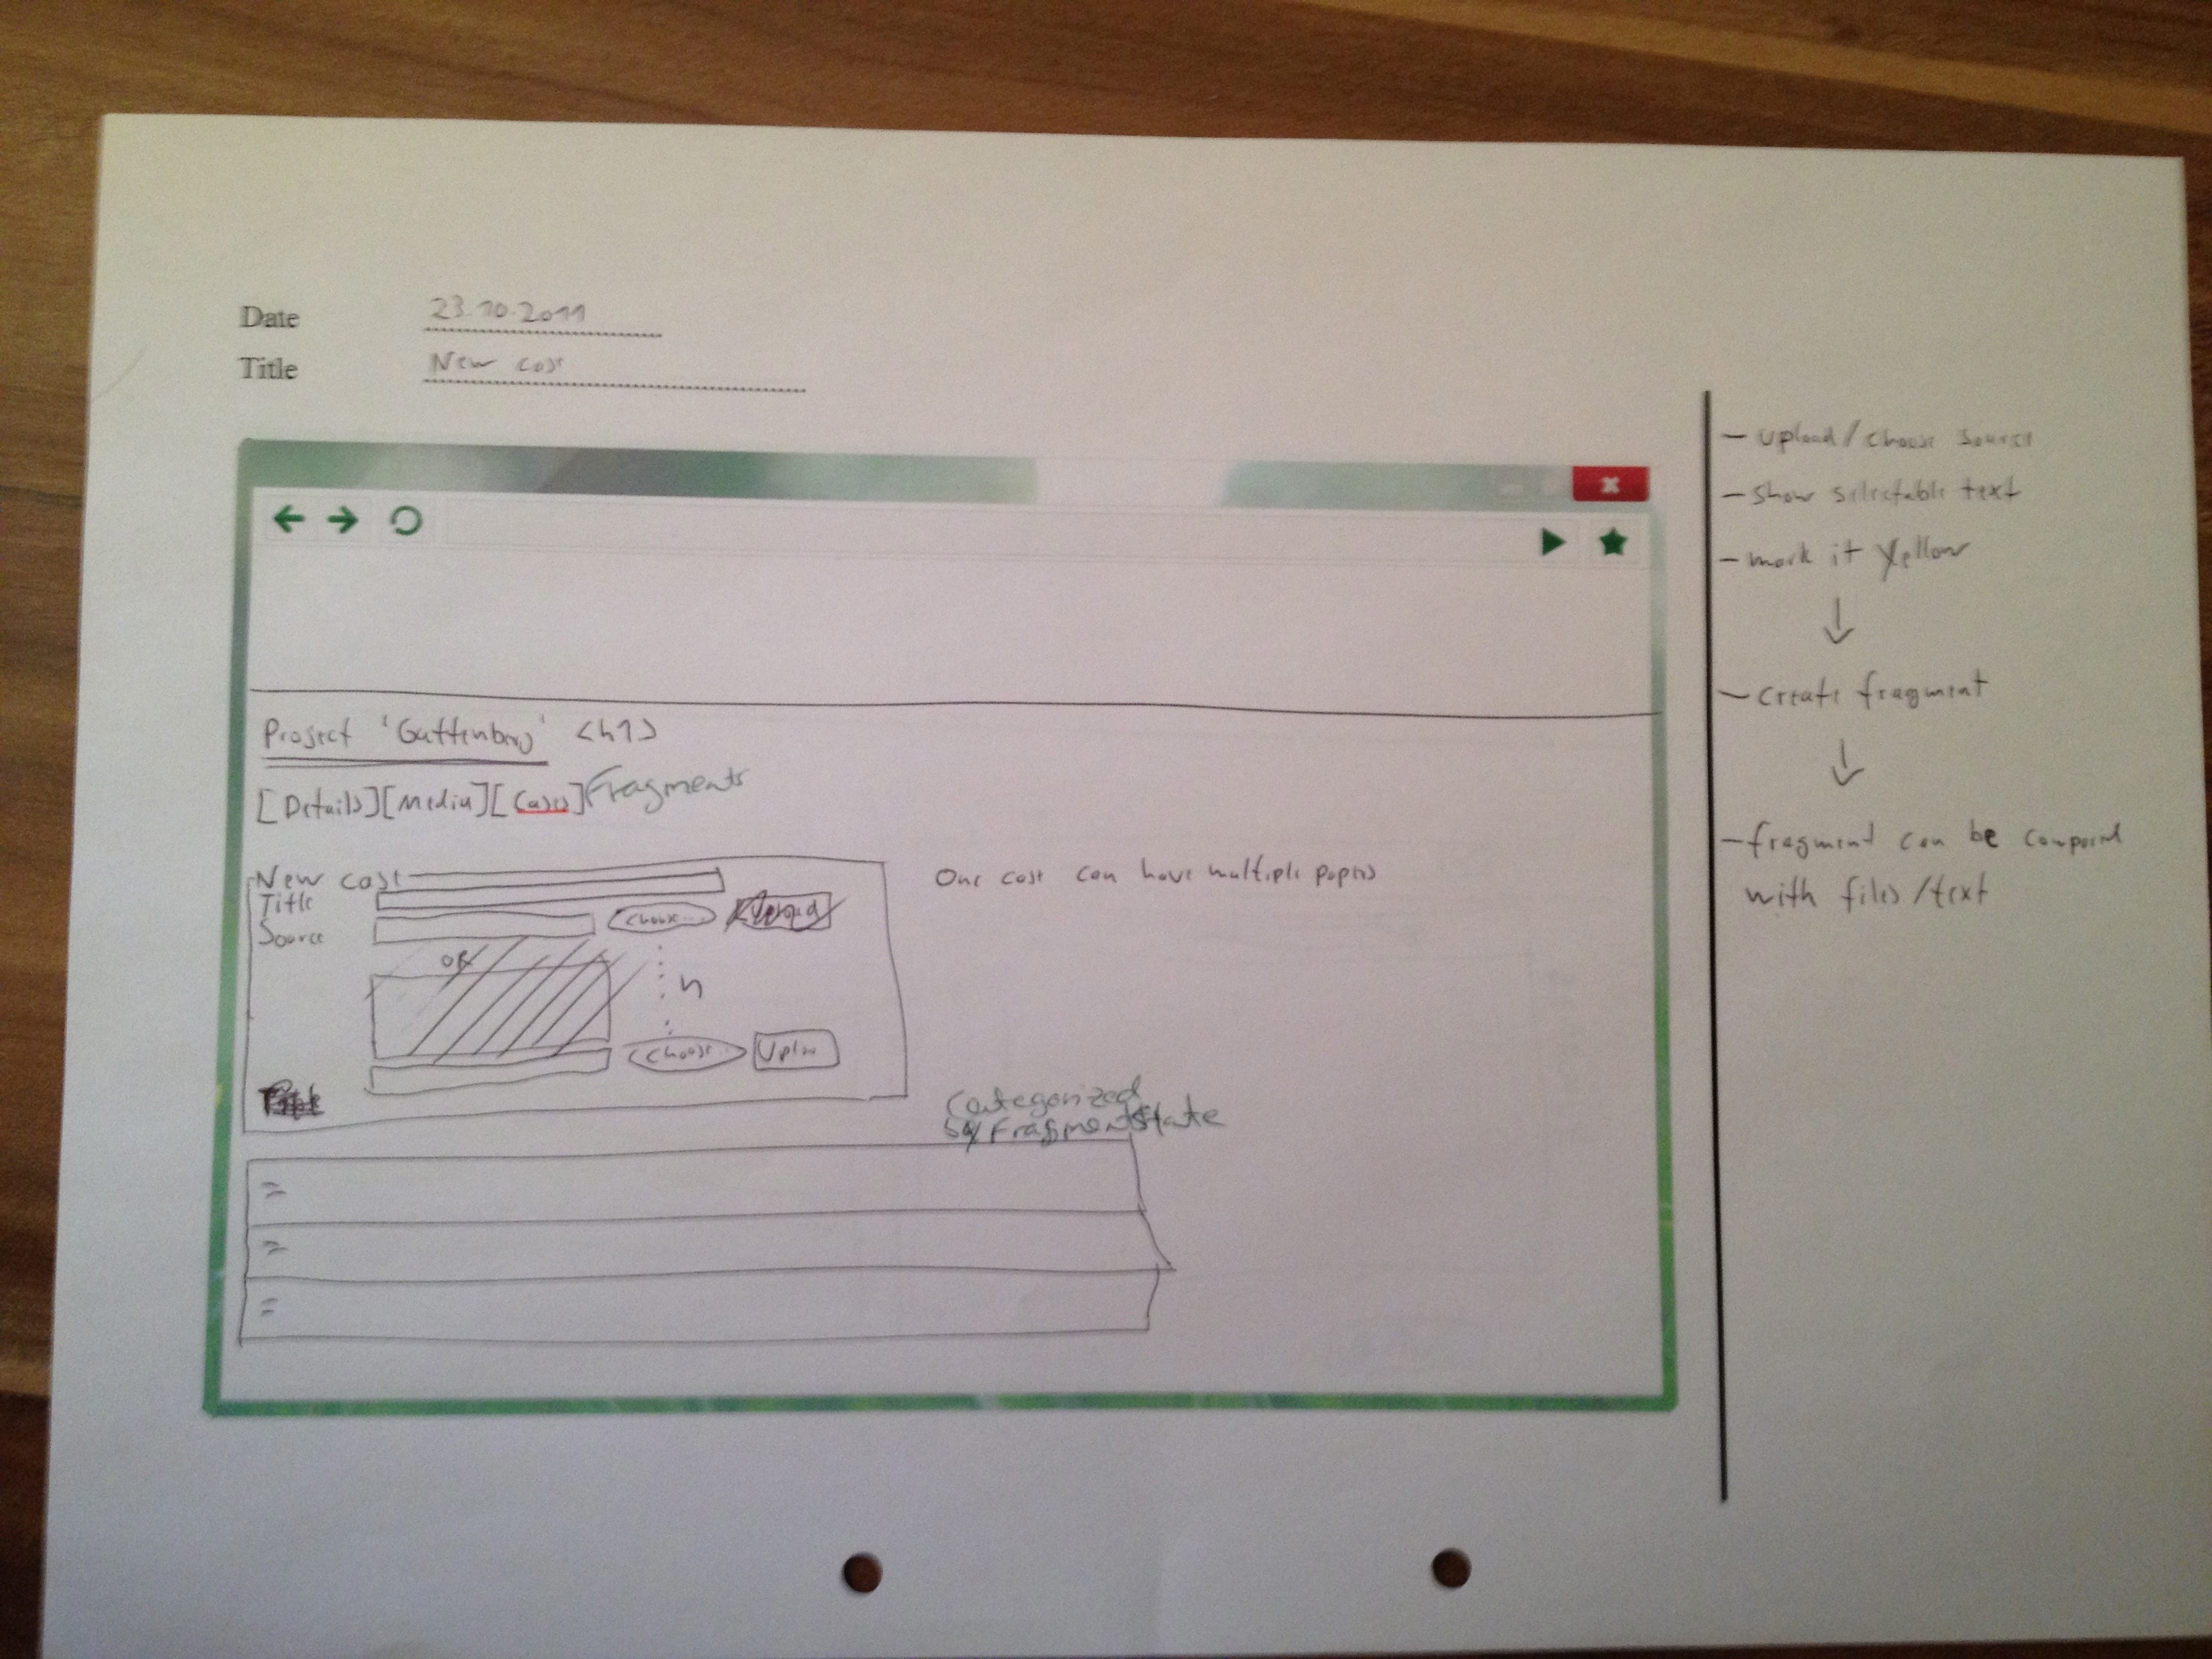
\includegraphics[width=\textwidth]{mockups/m_new_case.jpg}
  \caption{Mockup – New case – digitalized }
  \label{fig:1newCaseMockup}
\end{figure}

\begin{figure}[tbp]
  \centering
    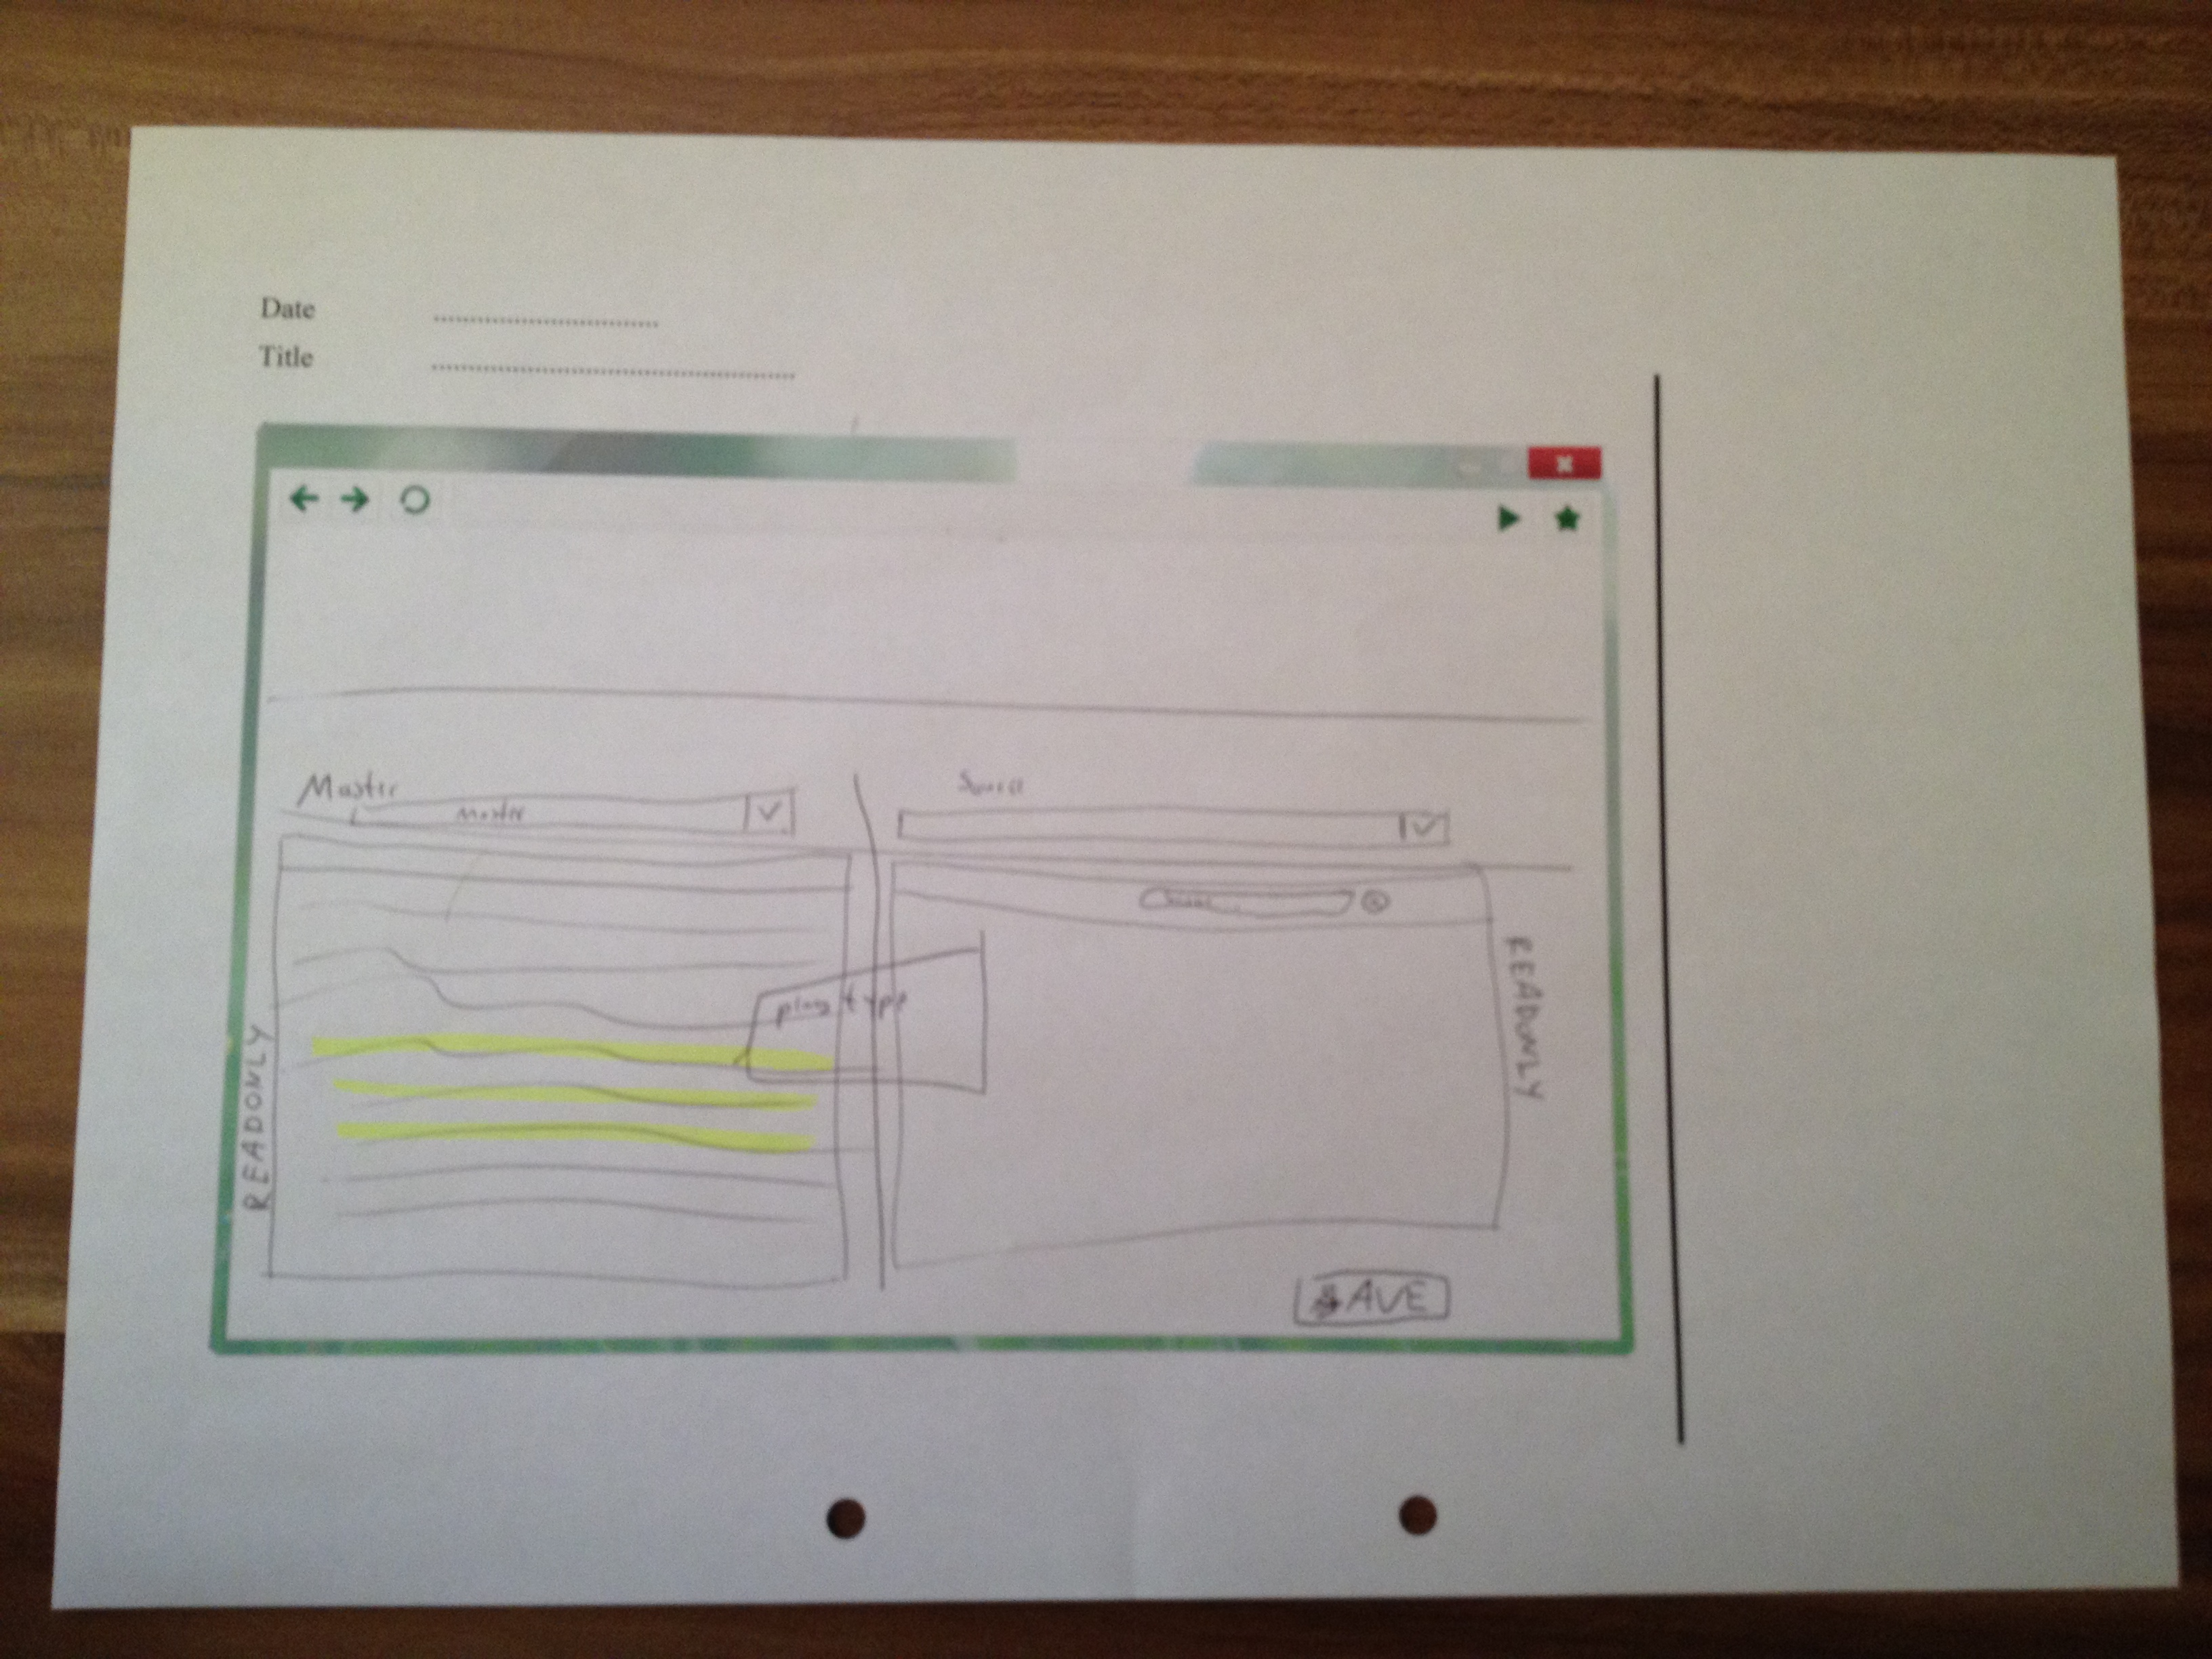
\includegraphics[width=\textwidth]{mockups/m_new_fragment.jpg}
  \caption{Mockup – New fragment – digitalized }
  \label{fig:1newCaseMockup}
\end{figure}

\begin{figure}[tbp]
  \centering
    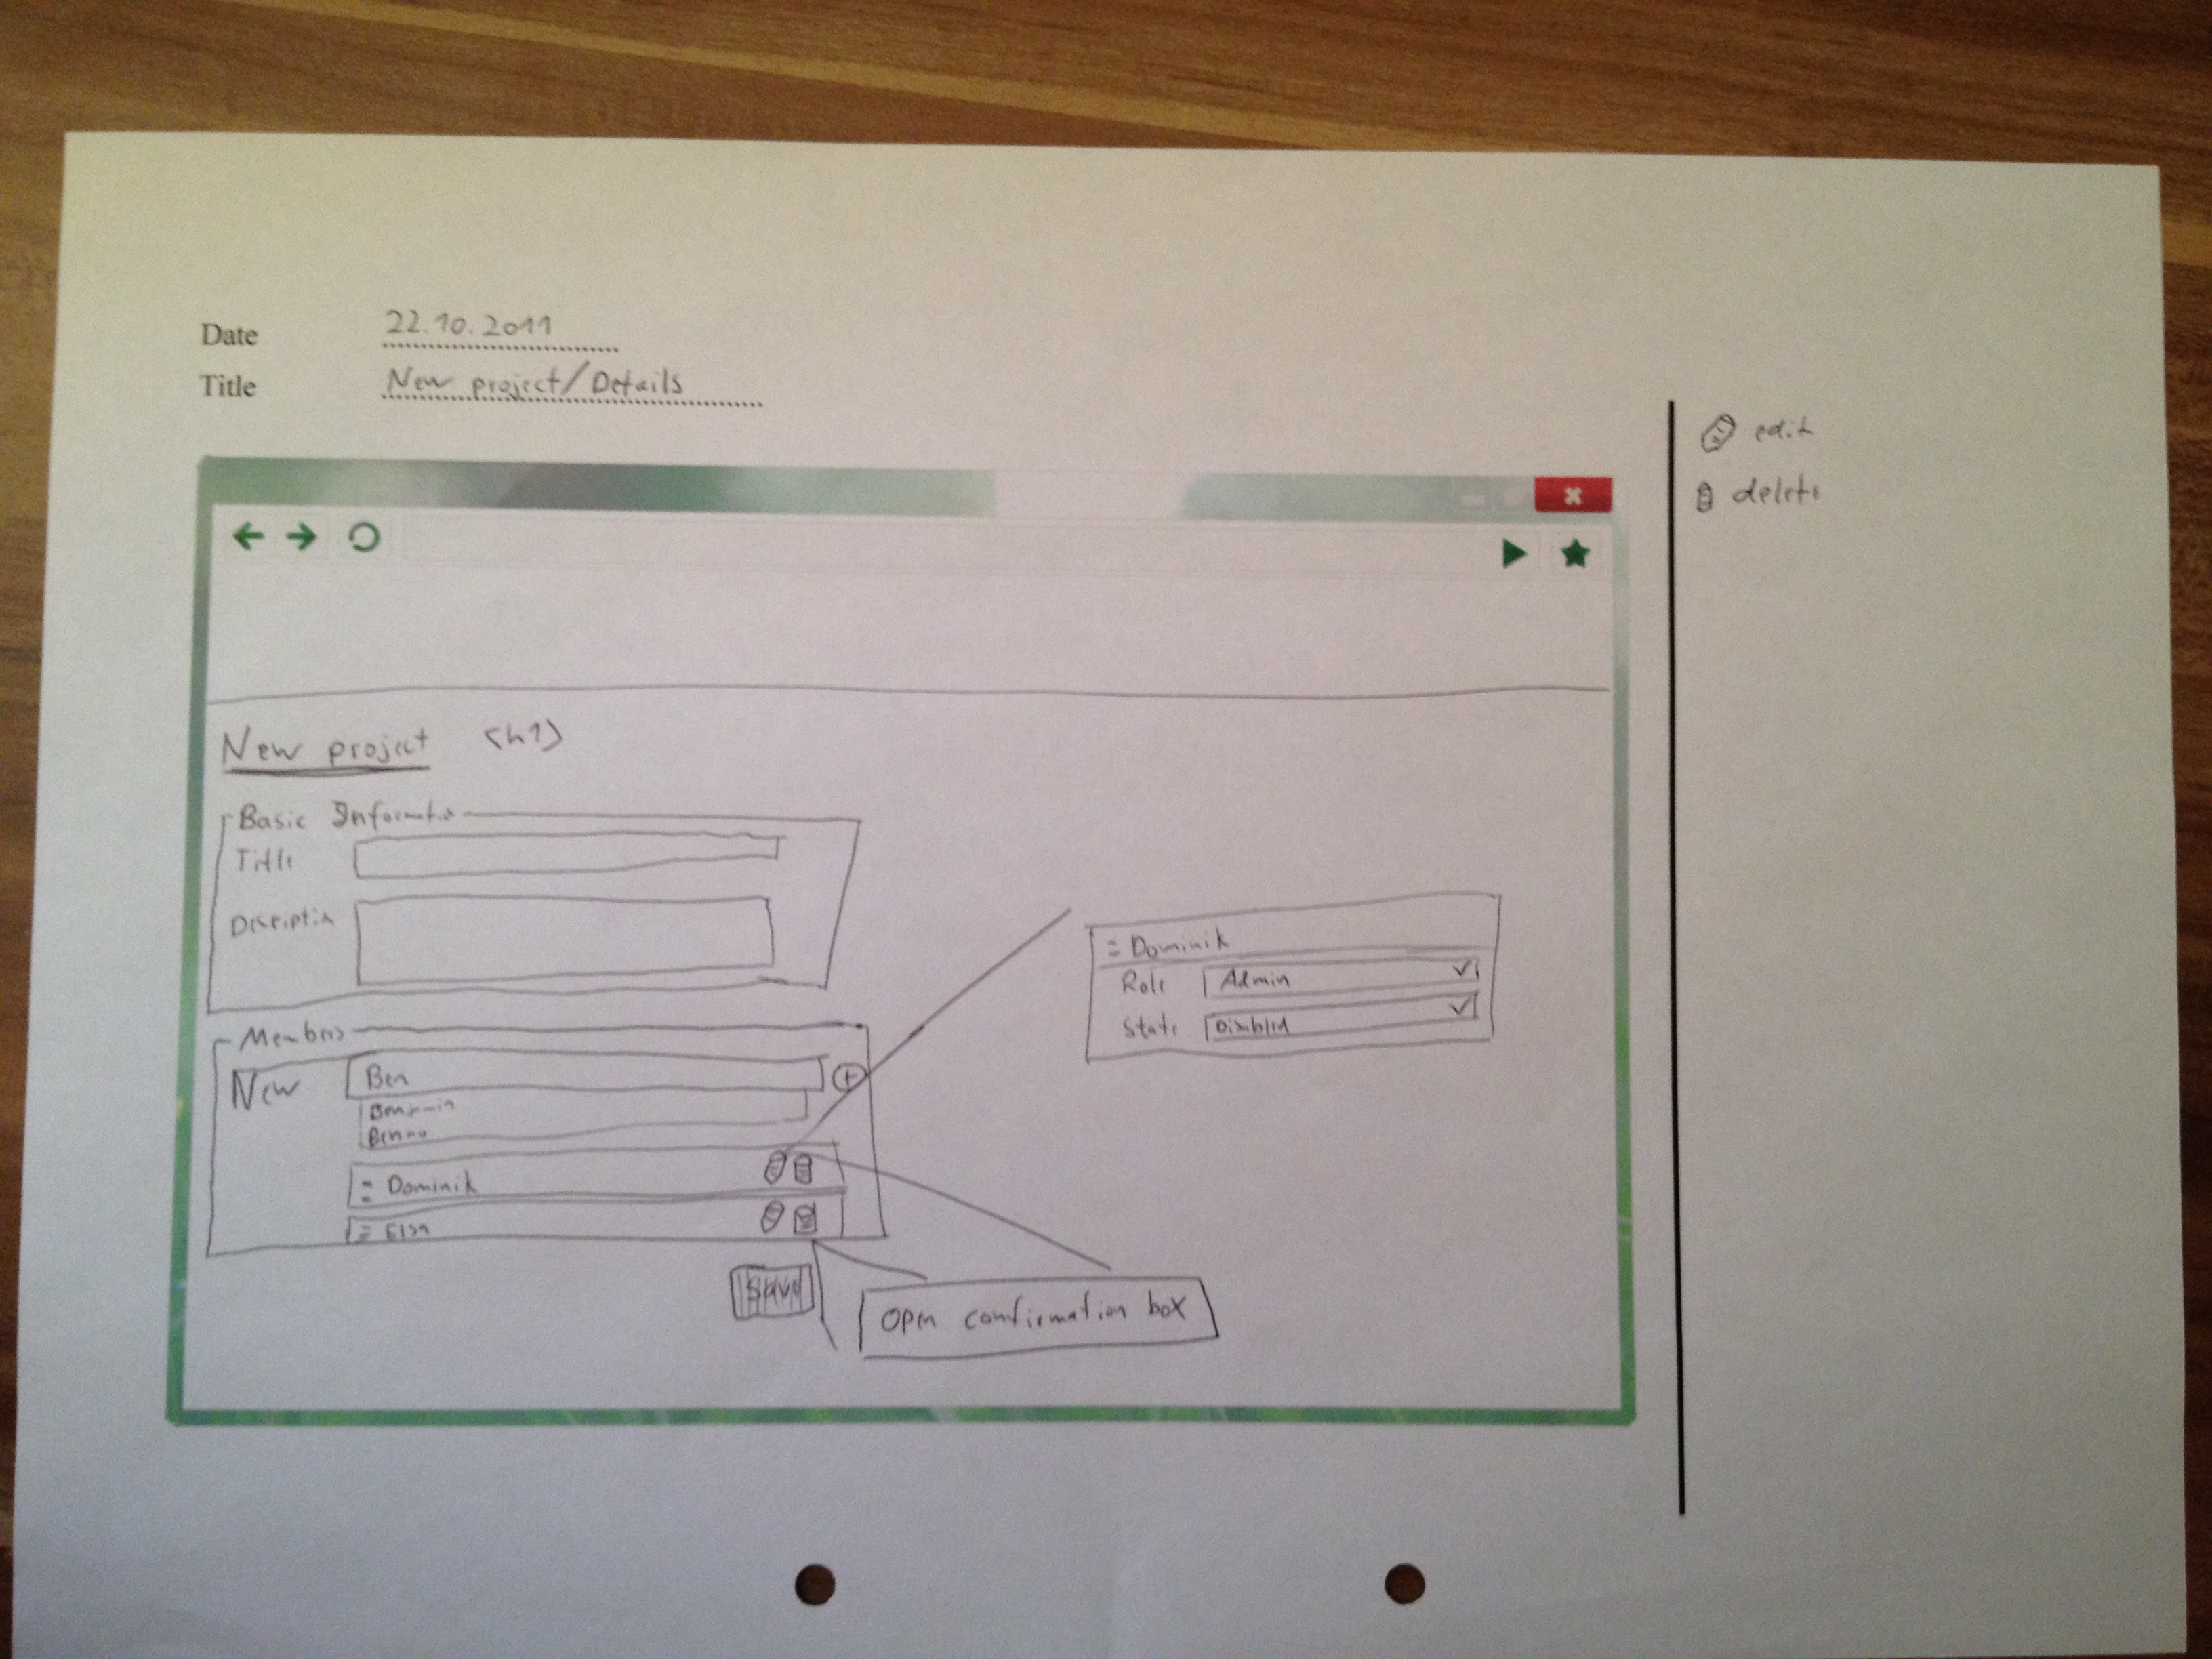
\includegraphics[width=\textwidth]{mockups/m_new_project.jpg}
  \caption{Mockup – New project – digitalized }
  \label{fig:mNewProjectMockup}
\end{figure}

\clearpage
\section{Digitalized}

\begin{figure}[tbp]
  \centering
    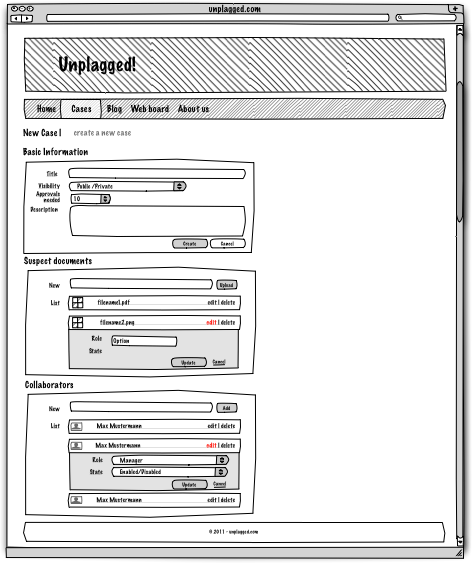
\includegraphics[width=0.86\textwidth]{mockups/1_new_case.png}
  \caption{Mockup – New case – digitalized }
  \label{fig:1newCaseMockup}
\end{figure}

\begin{figure}[tbp]
  \centering
    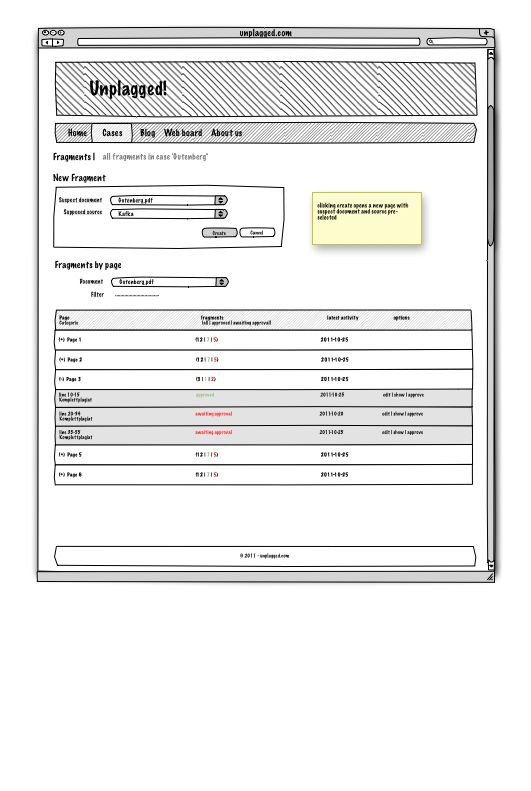
\includegraphics[width=\textwidth]{mockups/2_list_fragments.png}
  \caption{Mockup – List fragments – digitalized }
  \label{fig:2listFragmentsMockup}
\end{figure}

\begin{figure}[tbp]
  \centering
    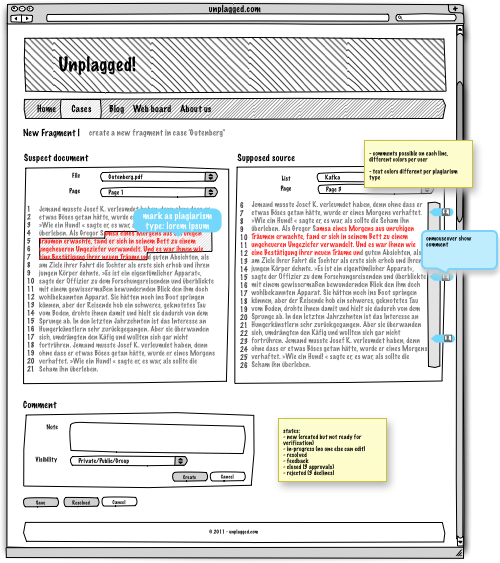
\includegraphics[width=\textwidth]{mockups/3_new_fragment.png}
  \caption{Mockup – New fragment – digitalized }
  \label{fig:3newFragmentMockup}
\end{figure}

\begin{figure}[tbp]
  \centering
    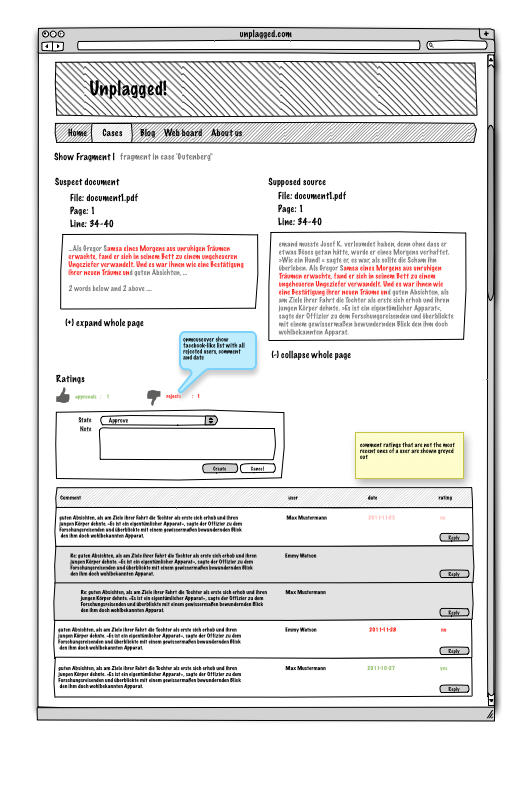
\includegraphics[width=0.97\textwidth]{mockups/4_show_fragment_for_approval.png}
  \caption{Mockup – Show fragment for approval – digitalized }
  \label{fig:4showFragmentForApprovalMockup}
\end{figure}

\begin{figure}[tbp]
  \centering
    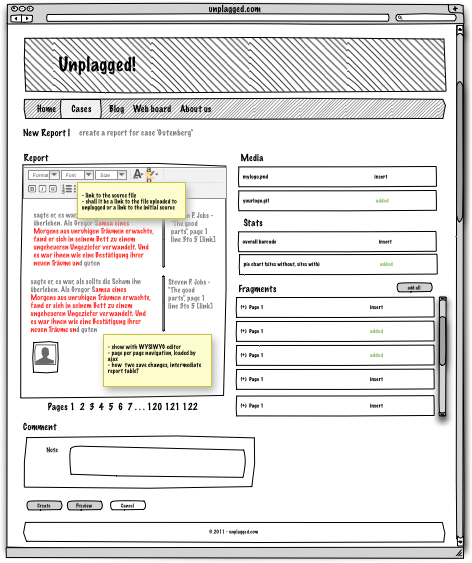
\includegraphics[width=\textwidth]{mockups/5_new_report.png}
  \caption{Mockup – New report – digitalized }
  \label{fig:5newReportMockup}
\end{figure}

\end{appendix}
